\begin{center}
    \section{Семинар IV}
\end{center}
\subsection{Решение задач на потенциальные ямы}
\excersize{Упражнение №13}{darklavender}
\begin{center}
    \textit{Найдите уровни энергии и волновые функции стационарных состояний для частицы m в одномерной потенциальной яме следующего вида:}
    \[
    U(x) =
    \begin{cases}
    +\infty,& x<0,\\
    -U_0,& 0<x<a,\\
    0,& x>a
    \end{cases}
    \]
\end{center}

На рисунке \ref{fig 4.1} можем увидеть потенциальную яму, но уже с бесконечной стенкой. Давайте обсудим, как от этого изменится задача.
\begin{figure}[!ht]
\centering
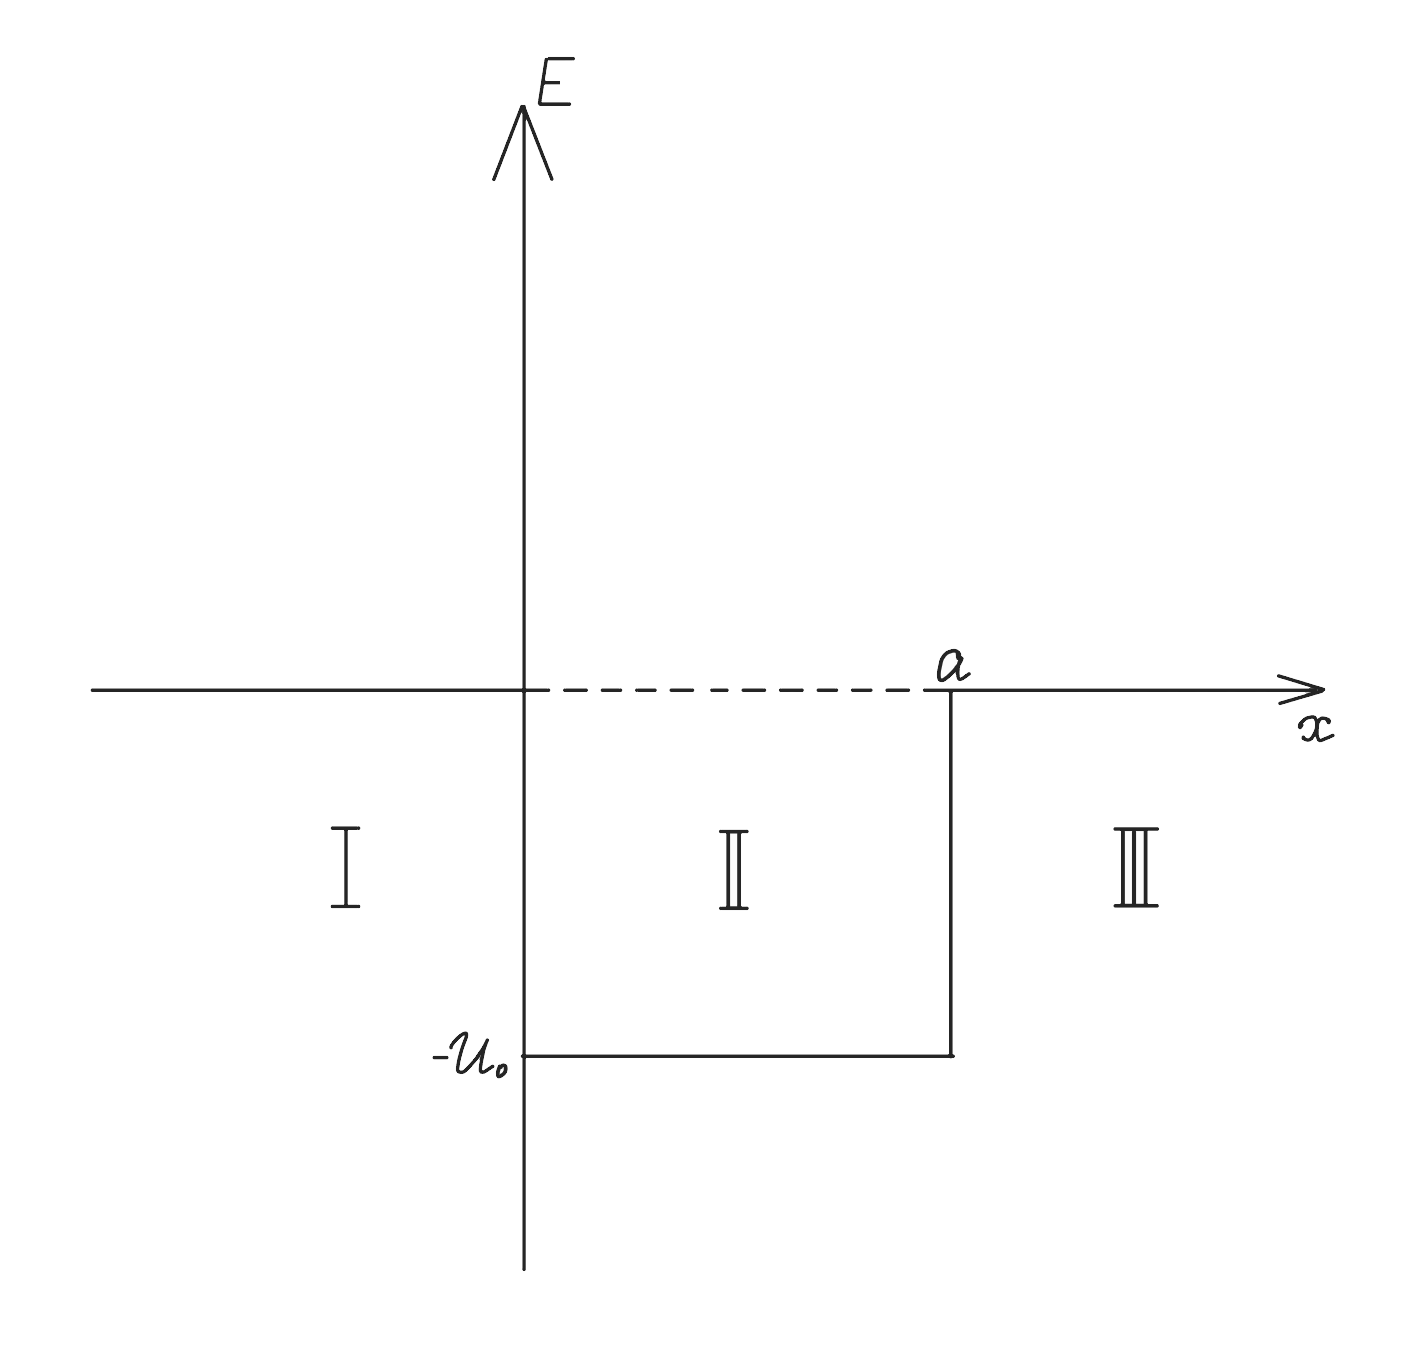
\includegraphics[scale=0.27]{class_4/images/half-inf hole.png}
\caption{Потенциальная яма с одной бесконечной стенкой}
\label{fig 4.1}
\end{figure}

Запишем уравнение Шрёдингера:
\[
\psi'' + \frac{2m}{\hbar^2}(E-U(x))\psi = 0 
\]
Заметим, что правая часть ямы очень похожа на яму из упражнения 12. Рассмотрим, что происходит у левой стенки. Мы считаем, что частица не может пройти через такой бесконечный барьер, то есть $\psi(x) = 0$ при $x\leq 0$. Тогда, из условия непрерывности, получим условия ``сшивки'' (напоминаю, что решения в области $II$ имеет вид $\psi(x) = \widetilde{A}\cos kx + A\sin kx$):
\[
\psi(0) = \widetilde{A} = 0 \implies \psi(x) =
\begin{cases}
    0,& x \leq 0,\\
    A\sin kx,& 0<x<a,\\
    Be^{-\kappa x},& x\geq a
\end{cases}
\]
Я думаю, уже видно, что мы можем переписать это через нечетные волновые функции из задачи 1.1. Тогда получим:
\[
\psi(x) =
\begin{cases}
    0, & x\leq 0,\\
    \sqrt{2}\psi_-(x), & x>0
\end{cases}
\]
Коэффициент $\sqrt{2}$ появился из следующих соображений: волновая функция, относительно первой задачи, уменьшилась вдвое, значит нужно её перенормировать. Если хотите в этом убедиться, подставьте вместо корня из двух коэффициент $C$ и решите уравнение $\int\limits_0^{+\infty}|\psi(x)|^2 = 1$.
\csquare{darklavender}

\excersize{Упражнение №14}{darklavender}
\begin{center}
    \textit{Частица массы m совершает финитное движение в одномерной модельной потенциальной яме, вид которой может быть представлен $\delta$-функцией:}
    \[
    U(x) = -\frac{\hbar^2\kappa_0}{m}\delta(x),
    \]
    \textit{где $\kappa_0$ - параметр ямы. Покажите, что в этой яме имеется только одно связанное состояние и найдите энергию и волновую функцию частицы связанного состояния в координатном представлении. Вычислите $\langle x\rangle,\,\langle p\rangle,\,\langle (\Delta x)^2\rangle$ и $\langle (\Delta p)^2\rangle$ в этом состоянии}
\end{center}

Не переживайте, дельта функция только выглядит страшно. На деле у нас получается примерно такой рисунок:
\begin{figure}[!ht]
\centering
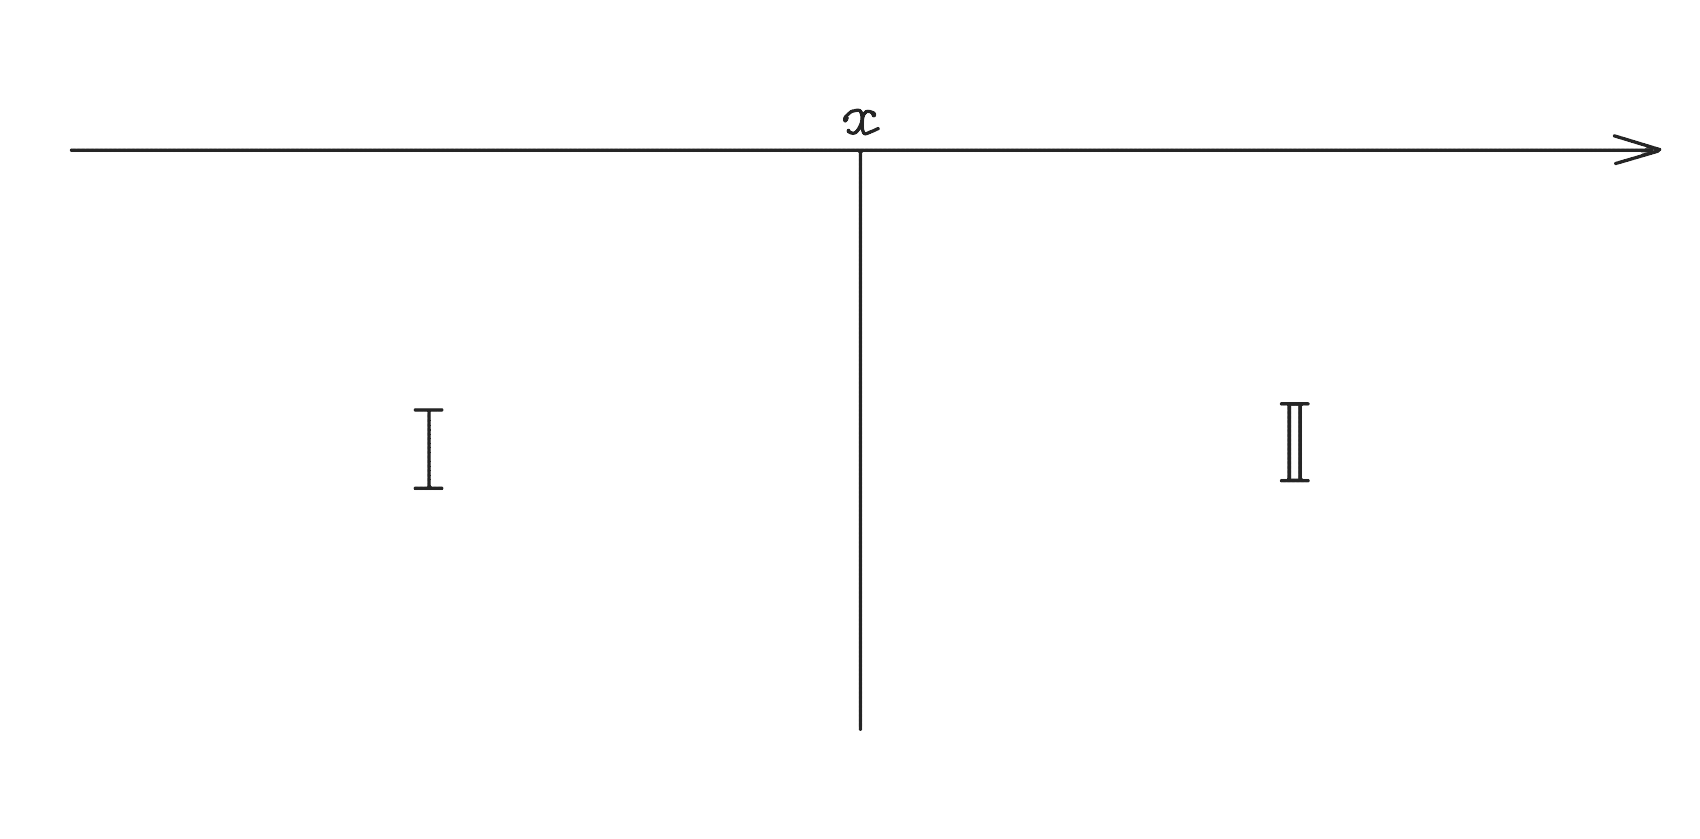
\includegraphics[scale=0.26]{class_4/images/delta hole.png}
\caption{Потенциальная дельта яма}
\label{fig 4.2}
\end{figure}\\
Введём уже знакомую нам величину $\kappa^2 = \frac{2m}{\hbar^2}|E|$ и запишем уравнение Шрёдингера:
\[
\psi''(x) - (\kappa^2 - 2\kappa_0\delta(x))\psi(x) = 0
\]
С областями такого типа, как I и II мы встречаемся уже третий раз, так что сразу выпишу их волновые функции:
\[
\begin{cases}
    \psi_I(x) = Ae^{\kappa x}\\
    \psi_{II}(x) = Be^{-\kappa x}\\
\end{cases}
\]

Волновая функция в нуле должна быть непрерывна: 
\begin{equation}
\psi(+0) = \psi(-0)    
\end{equation}
Производная же будет разрывна (из-за дельта-функции). Доопределим разрыв, проинтегрировав уравнение Шрёдингера с пределами от $-\epsilon$ до $\epsilon$, где $\epsilon \rightarrow 0$. Получим:
\begin{gather*}
\int\limits_{-\epsilon}^{\epsilon}\psi''(x)dx = \int\limits_{-\epsilon}^{\epsilon}\psi(x)\kappa^2 dx - \int\limits_{-\epsilon}^{\epsilon}2\kappa_0\delta(x)\psi(x) dx \implies\\
\implies \psi'(+0) - \psi'(-0) = -2\kappa_0\psi(0)    
\end{gather*}
Второй интеграл равен нулю, так как по теореме о среднем этот интеграл равен $2\mu\epsilon$, но $\epsilon \rightarrow 0$.

Выпишем волновые функции и воспользуемся полученными условиями:
\[
\begin{cases}
    \psi_I(x) = Ae^{\kappa x}\\
    \psi_{II}(x) = Be^{-\kappa x}\\
    \psi(+0) = \psi(-0)
\end{cases}
\implies A = B \implies \psi(x) = Ae^{-\kappa|x|}
\]
Подставим условие на производную и получим:
\[
-A\kappa - A\kappa = -2A\kappa_0 \implies \kappa = \kappa_0 
\]
Тогда, можно явно выразить энергию через заданное нам условием значение $\kappa_0$:
\[
E_0 = - \frac{\hbar^2 \kappa_0^2}{2m}
\]
Выходит, что в дельта яме только один уровень энергии. Найдём коэффициент A из условия нормировки:
\begin{gather*}
\int\limits_{-\infty}^{+\infty} |\psi(x)|^2 dx = A^2\int\limits_{-\infty}^{+\infty} e^{-2\kappa |x|} = A^2\left[\int\limits_{-\infty}^0 e^{2\kappa x} + \int\limits_0^{+\infty} e^{-2\kappa x}\right] =\\
= A^2\left[ \frac{1}{2\kappa}(1 - 0) - \frac{1}{2\kappa}(0-1)\right] = \frac{A^2}{\kappa} = 1 \implies  \\ \implies  A = \sqrt{\kappa}
\end{gather*}


Наконец, запишем итоговую волновую функцию:
\[
\psi(x) = \sqrt{\kappa_0}e^{-\kappa_0 |x|}
\]
Найдём среднее значение координаты и импульса. Дисперсию читателю представляется найти самостоятельно в виде упражнения.
\[
\langle x \rangle = \int\psi^*x\psi dx = 0, \text{т.к. $\psi$ - чётная}
\]
\[
\langle p \rangle = \int\psi^*(-i\hbar\frac{\partial}{\partial x}\psi) dx = -i\hbar\kappa_0^2\int e^{-\kappa_0|x|}(-e^{-\kappa_0|x|}sign(x)) dx = 0
\]
\csquare{darklavender}
\excersize{Упражнение №15}{darklavender}
\begin{center}
    \textit{Частица массы m совершает финитное движение в одномерном потенциальном поле вида:}
    \[
    U(x) = -\frac{\hbar^2\kappa_0}{m}(\delta(x+a) + \delta(x-a)),
    \]
    \textit{где $\kappa_0$ - параметр ямы. Найдите энергии уровней и волновые функции стационарных состояний. Как зависит число связанных состояний от параметров $a$ и $\kappa_0$?}
    
    \textit{Покажите, что в случае $\kappa_0a \gg 1$ связанные состояния представляют собой дублет близко расположенных уровней}
\end{center}

На рисунке \ref{fig 4.3} можно увидеть ситуацию, описываемую в задаче.
\begin{figure}[!ht]
\centering
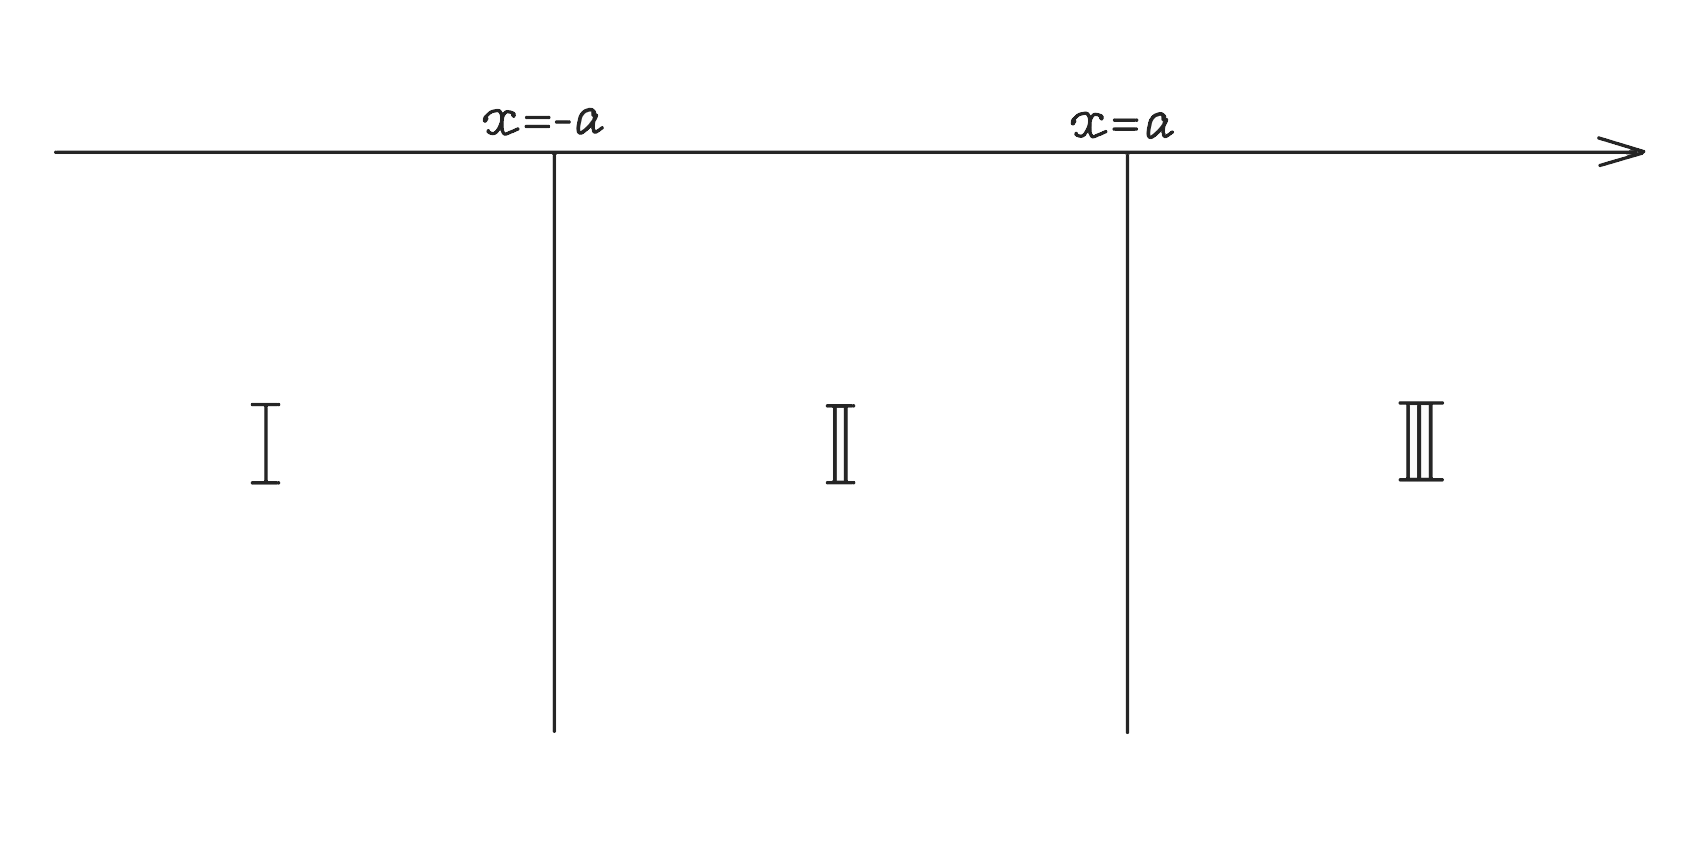
\includegraphics[scale=0.27]{class_4/images/two delta hole.png}
\caption{Две потенциальные дельта ямы}
\label{fig 4.3}
\end{figure}

Давайте для начала рассмотрим области вне дельта ям. Ясно (если нет, проделайте те же самые выкладки, что мы делали в задаче 1.1), что решением здесь будут так же четные и нечетные функции следующего вида:
\[
\psi_+ =
\begin{cases}
    Ae^{\kappa x}, & x < -a,\\
    B\,ch\,\kappa x, & -a < x < a,\\
    Ae^{-\kappa x},& x > a
\end{cases}\quad
\psi_- =
\begin{cases}
    -De^{\kappa x},& x < -a,\\
    C\, sh\, \kappa x, & -a < x < a,\\
    De^{-\kappa x},& x > a
\end{cases}
\]
Тригонометрические функции превратились в гиперболические из-за отсутствия отрицательного потенциала между ямами. Далее, приведём к форме, удобной для анализа (в очередной раз графического). Для этого вновь воспользуемся условиями ``сшивки'', а именно разрывом производной и непрерывностью, полученной в прошлой задаче:
\[
\begin{cases}
\psi'(a+0) - \psi'(a-0) = -2\kappa_0\psi(a)\\
\psi(a+0) = \psi(a-0)    
\end{cases}
\]
Проведем все необходимые преобразования для чётных функций (для нечётных аналогично):
\[
Ae^{-\kappa a} = B\,ch\,ka => B = \frac{1}{2}A(e^{2\kappa a} + 1)
\]
Из первого уравнения получим:
\[
-A\kappa e^{-\kappa a} - B\kappa\,\sh\,\kappa a = -2\kappa_0 Be^{-\kappa a}
\]
Подставляя $B$ и проведя все сокращения, получим итоговое выражение:
\begin{equation}
    \frac{\kappa a}{\kappa_0 a} = 1 + e^{-2\kappa a}
\end{equation}
Для нечетного же случая:
\begin{equation}
    \frac{\kappa a}{\kappa_0 a} = 1 - e^{-2\kappa a}
\end{equation}
Давайте опять сделаем красивый (или не очень) график и обсудим его.
\begin{figure}[!ht]
\centering
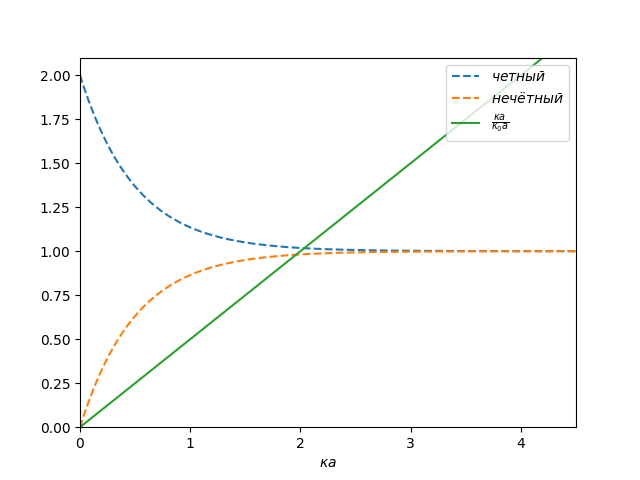
\includegraphics[scale=0.7]{class_4/images/delta.png}
\caption{График для нечетных и четных функций}
\label{fig 4.4}
\end{figure}

Два важных замечания по графику:
\begin{enumerate}
    \item Видно, что чётное решение, в отличие от нечётного, существует всегда. Нечётное решение же существует только при $\kappa_0a\geq 1/2$.
    \item При $\kappa_0a\gg 1$ решения почти неразличимы. Однако, если $\kappa a \ll 1$, то у нас остаётся одна дельта яма с удвоенным $\kappa_0$.
\end{enumerate}
Найдём коэффициенты для собственных функций (так же, как в упражнении 12).
\[
|A|^2 =  (a + \frac{sh\, 2\kappa a}{2\kappa} + \frac{ch ^2\,\kappa a}{\kappa})^{-1},\; B = Ae^{\kappa a}\,ch\,\kappa a
\]
\[
|D|^2 = (-a + \frac{sh\, 2\kappa a}{2\kappa} + \frac{sh ^2\,\kappa a}{\kappa})^{-1},\;C = De^{\kappa a}\,sh\,\kappa a
\]
\csquare{darklavender}

\excersize{Упражнение №16}{darklavender}
\begin{center}
    \textit{Частица массы m движется в одномерном периодическом поле вида}
    \[
    U(x) = -\frac{\hbar^2\kappa_0}{m}\sum\limits_{n=-\infty}^{n = +\infty}\delta(x-na),
    \]
    \textit{где $\kappa_0$ и $a$ - параметры потенциала. Исследуйте, при каких отрицательных и положительных энергиях $E$ частицы такое движение возможно. Покажите, что имеются зоны ``разрешенных'' и ``запрещенных'' энергий.}
    \textit{Исследуйте, что происходит с шириной зон в предельных случаях $\kappa_0a\gg1$ (сильная связь) и $\kappa_0a\ll1$(слабая связь).}
    
\end{center}

Мы решили задачу на одну яму, на две ямы, следующий логичный шаг - решить задачу на \sout{три} бесконечность дельта ям.

Писать условие сшивки для бесконечного количества ям не самая приятная задача и предоставляется читателю в качестве упражнения на дом. Мы же пойдём другим путём, заметив важную особенность задачи. Посмотрев на рисунок \ref{fig 4.5} и на дельта потенциал, становится понятно, что задача a-периодична. А какой оператор у нас двигает частицу на a? Правильно, оператор трансляции $\hat{T}_a$. Проверим, коммутирует ли гамильтониан с оператором трансляции:
\[
[\hat{H}, \hat{T}_a] = [U(x), \hat{T}_a] + [\hat{p}^2, \hat{T}_a] = [\sum\delta(x-na), \hat{T}_a] + [\hat{p}^2, e^{-\frac{i}{\hbar}a\hat{p}}] = 0.
\]
Значит, мы можем искать собственные функции гамильтониана в виде $e^{ikx}\phi(x)$, где $\phi(x + a) = \phi(x)$. Помимо этого, нам достаточно написать условия сшивки для зоны I и зоны II. Теперь, когда мы знаем, что волновые функции для задачи являются собственными для оператора трансляции, можем выписать действие оператора трансляции отдельно:
\[
\hat{T}_a\psi(x) = \psi(x+a) = e^{ia\kappa}\psi(x)
\]
\begin{figure}[!ht]
\centering
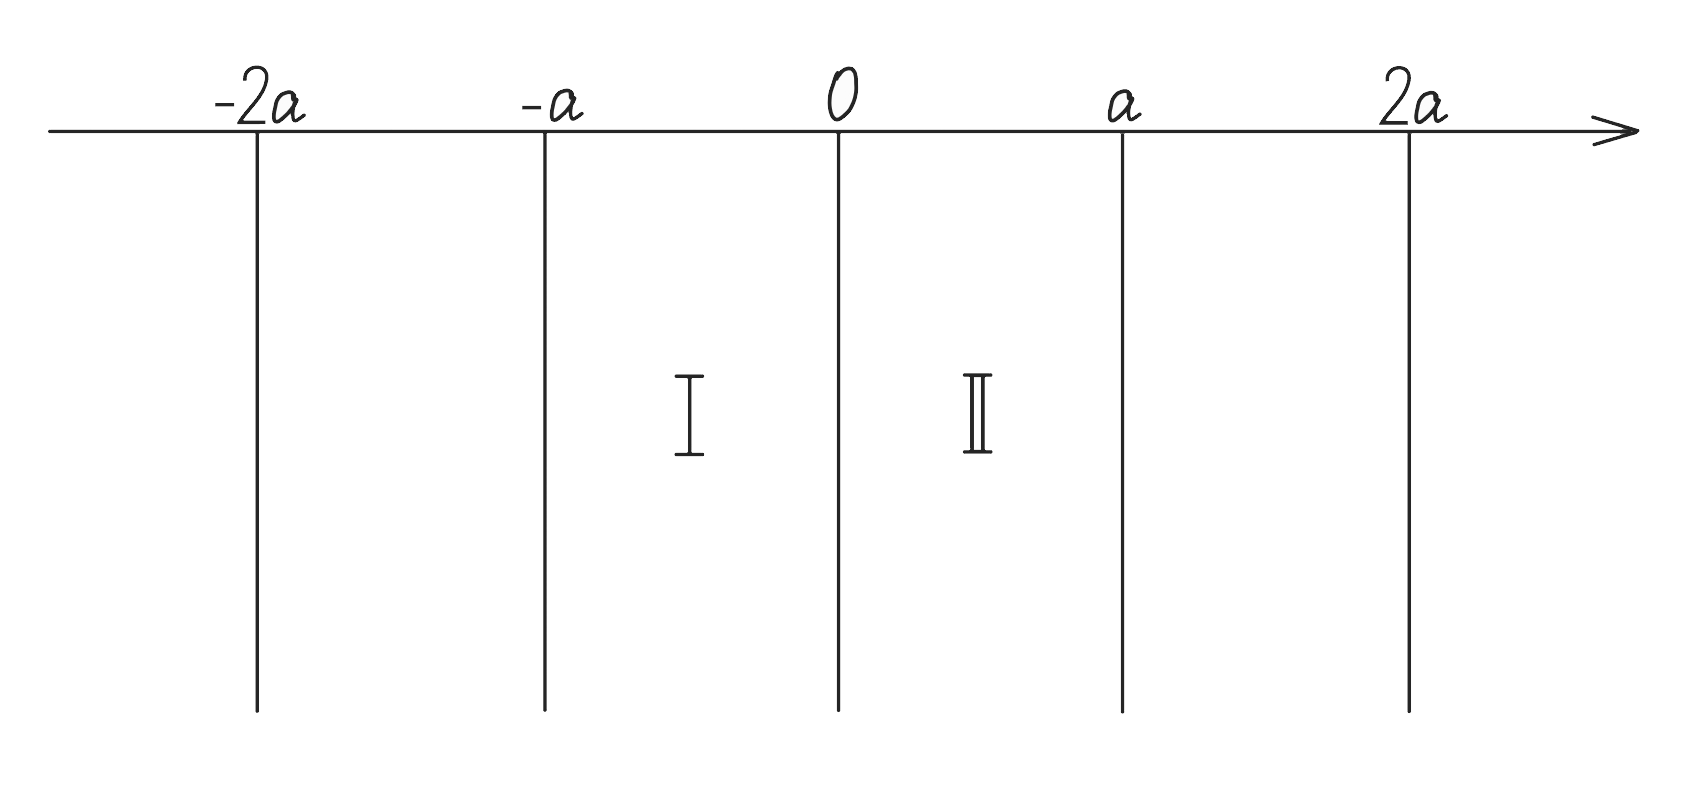
\includegraphics[scale=0.27]{class_4/images/inf delta hole.png}
\caption{Бесконечные дельта ямы}
\label{fig 4.5}
\end{figure}

Напишем уравнение Шрёдингера для зоны I и зоны II без учёта дельта потенциала и с положительной энергией (!):
\[
\psi''(x) + \kappa^2\psi(x) = 0, \; \kappa^2 = \frac{2m}{\hbar^2}E
\]
Решение в первой области мы знаем:
\[
\psi_I(x) = Ae^{i\kappa x} + Be^{-i\kappa x}
\]
Получим из него уравнение для второй области:
\[
\hat{T}_a\psi_I(x) = \psi_I(x+a) = \psi_{II}(x)
\]
Мы знаем, что волновые функции являются собственными для оператора трансляции. Тогда:
\[
\psi_{II}(x) = e^{ika}\psi_I(x-a) = e^{ika}(Ae^{i\kappa (x-a)} + Be^{-i\kappa (x - a)})
\]
Таким образом, мы смогли выразить оба наших решения через одни коэффициенты A и B.

Теперь запишем условия сшивки. Напомню, что $\psi_I(0) = \psi_{II}(0)$ и $\psi'_{II}(0) - \psi'_I(0) = -2\kappa_0\psi(0)$. Тогда
\[
\begin{cases}
A + B = e^{ika}\left[Ae^{-i\kappa a} + Be^{i\kappa a}\right]\\
e^{ika}(Ae^{-i\kappa a}i\kappa - Be^{i\kappa a}i\kappa) - Ai\kappa + Bi\kappa = -2\kappa_0(A+B)
\end{cases}
\]
Чтобы у системы уравнений было нетривиальное решение, необходимо, чтобы определитель матрицы системы был равен нулю. Давайте выпишем матрицу системы:
\begin{align*}
&\begin{cases}
A(1 - e^{i(k-\kappa)a}) + B(1 - e^{i(k+\kappa)a}) = 0\\
A(e^{i(k-\kappa)a}i\kappa - i\kappa + 2\kappa_0) - B(e^{i(k+\kappa)a}i\kappa - i\kappa - 2\kappa_0) = 0
\end{cases} \implies\\
\implies &\begin{vmatrix}
1 - e^{i(k-\kappa)a} & 1 - e^{i(k+\kappa)a} \\
e^{i(k-\kappa)a}i\kappa - i\kappa + 2\kappa_0 & e^{i(k+\kappa)a}i\kappa - i\kappa - 2\kappa_0
\end{vmatrix}
= 0
\end{align*}
Распишем детерминант и воспользуемся всей мощью тригонометрии:
\begin{align*}
(1 - e^{i(k-\kappa)a})&(e^{i(k+\kappa)a}i\kappa - i\kappa - 2\kappa_0) - (1 - e^{i(k+\kappa)a})(e^{i(k-\kappa)a}i\kappa - i\kappa + 2\kappa_0) = \\
 = &i\kappa - i\kappa e^{i(k-\kappa)a} - i\kappa e^{i(k+\kappa)a} + i\kappa e^{2ika} - \kappa_0 e^{i(k-\kappa)a} + \kappa_0 e^{i(k+\kappa)a} = \\
 = &e^{ika}\left( i\kappa e^{-ika} - i\kappa e^{-i\kappa a} - i\kappa e^{i\kappa a} + i\kappa e^{ika} - \kappa_0 e^{-i\kappa a} + \kappa_0 e^{i\kappa a}\right) = \\ 
 = &i\kappa\left( 2\cos ka - 2\cos\kappa a \right) + 2i\kappa_0\sin\kappa a =\\
 = &i\kappa\cos ka - i\kappa\cos\kappa a + i\kappa_0\sin\kappa a = 0
\end{align*}
В итоге получаем:
\[
\cos ka = \cos\kappa a - \frac{\kappa_0}{\kappa}\sin\kappa a
\]
Проделав то же самое для отрицательной энергии, получим:
\[
\cos ka = \cosh(\eta a) - \frac{\kappa_0}{\eta}\sinh(\eta a), \; \eta^2 = \frac{2m}{\hbar^2}|E|
\]
Мы получили зависимость энергии ($\kappa$ или $\eta$) от квазиимпульса $k$, т.е. у нас получились дисперсионные соотношения. Давайте проанализируем случай положительных энергий. Для этого преобразуем получившееся уравнение:
\begin{align*}
    \cos \kappa a - \frac{\kappa_0}{\kappa}\sin\kappa a & = \frac{\sqrt{(\kappa a)^2 + (\kappa_0 a)^2}}{\kappa}\left( \frac{\kappa}{\sqrt{(\kappa a)^2 + (\kappa_0 a)^2}}\cos \kappa a -  \frac{\kappa_0}{\sqrt{(\kappa a)^2 + (\kappa_0 a)^2}}\sin \kappa a\right) = \\
    & = \frac{\sqrt{(\kappa a)^2 + (\kappa_0 a)^2}}{a\kappa}\left( \frac{1}{\sqrt{1 + (\frac{\kappa_0}{\kappa})^2}}\cos \kappa a -  \frac{1}{\sqrt{(\frac{\kappa}{\kappa_0})^2 + 1}}\sin \kappa a\right) = \\
    & = \frac{\sqrt{(\kappa a)^2 + (\kappa_0 a)^2}}{a\kappa}\left( \cos\phi \cos\kappa a -  \sin\phi\sin \kappa a\right), \phi = \arctan \frac{\kappa_0}{\kappa} =\\
    & =  \frac{\sqrt{(\kappa a)^2 + (\kappa_0 a)^2}}{a\kappa}\cos (\kappa a + \phi)
\end{align*}

В итоге получим уравнение:
\[
\cos ka = \frac{\sqrt{(\kappa a)^2 + (\kappa_0 a)^2}}{a\kappa}\cos (\kappa a + \phi)
\]

\begin{figure}[!ht]
\centering
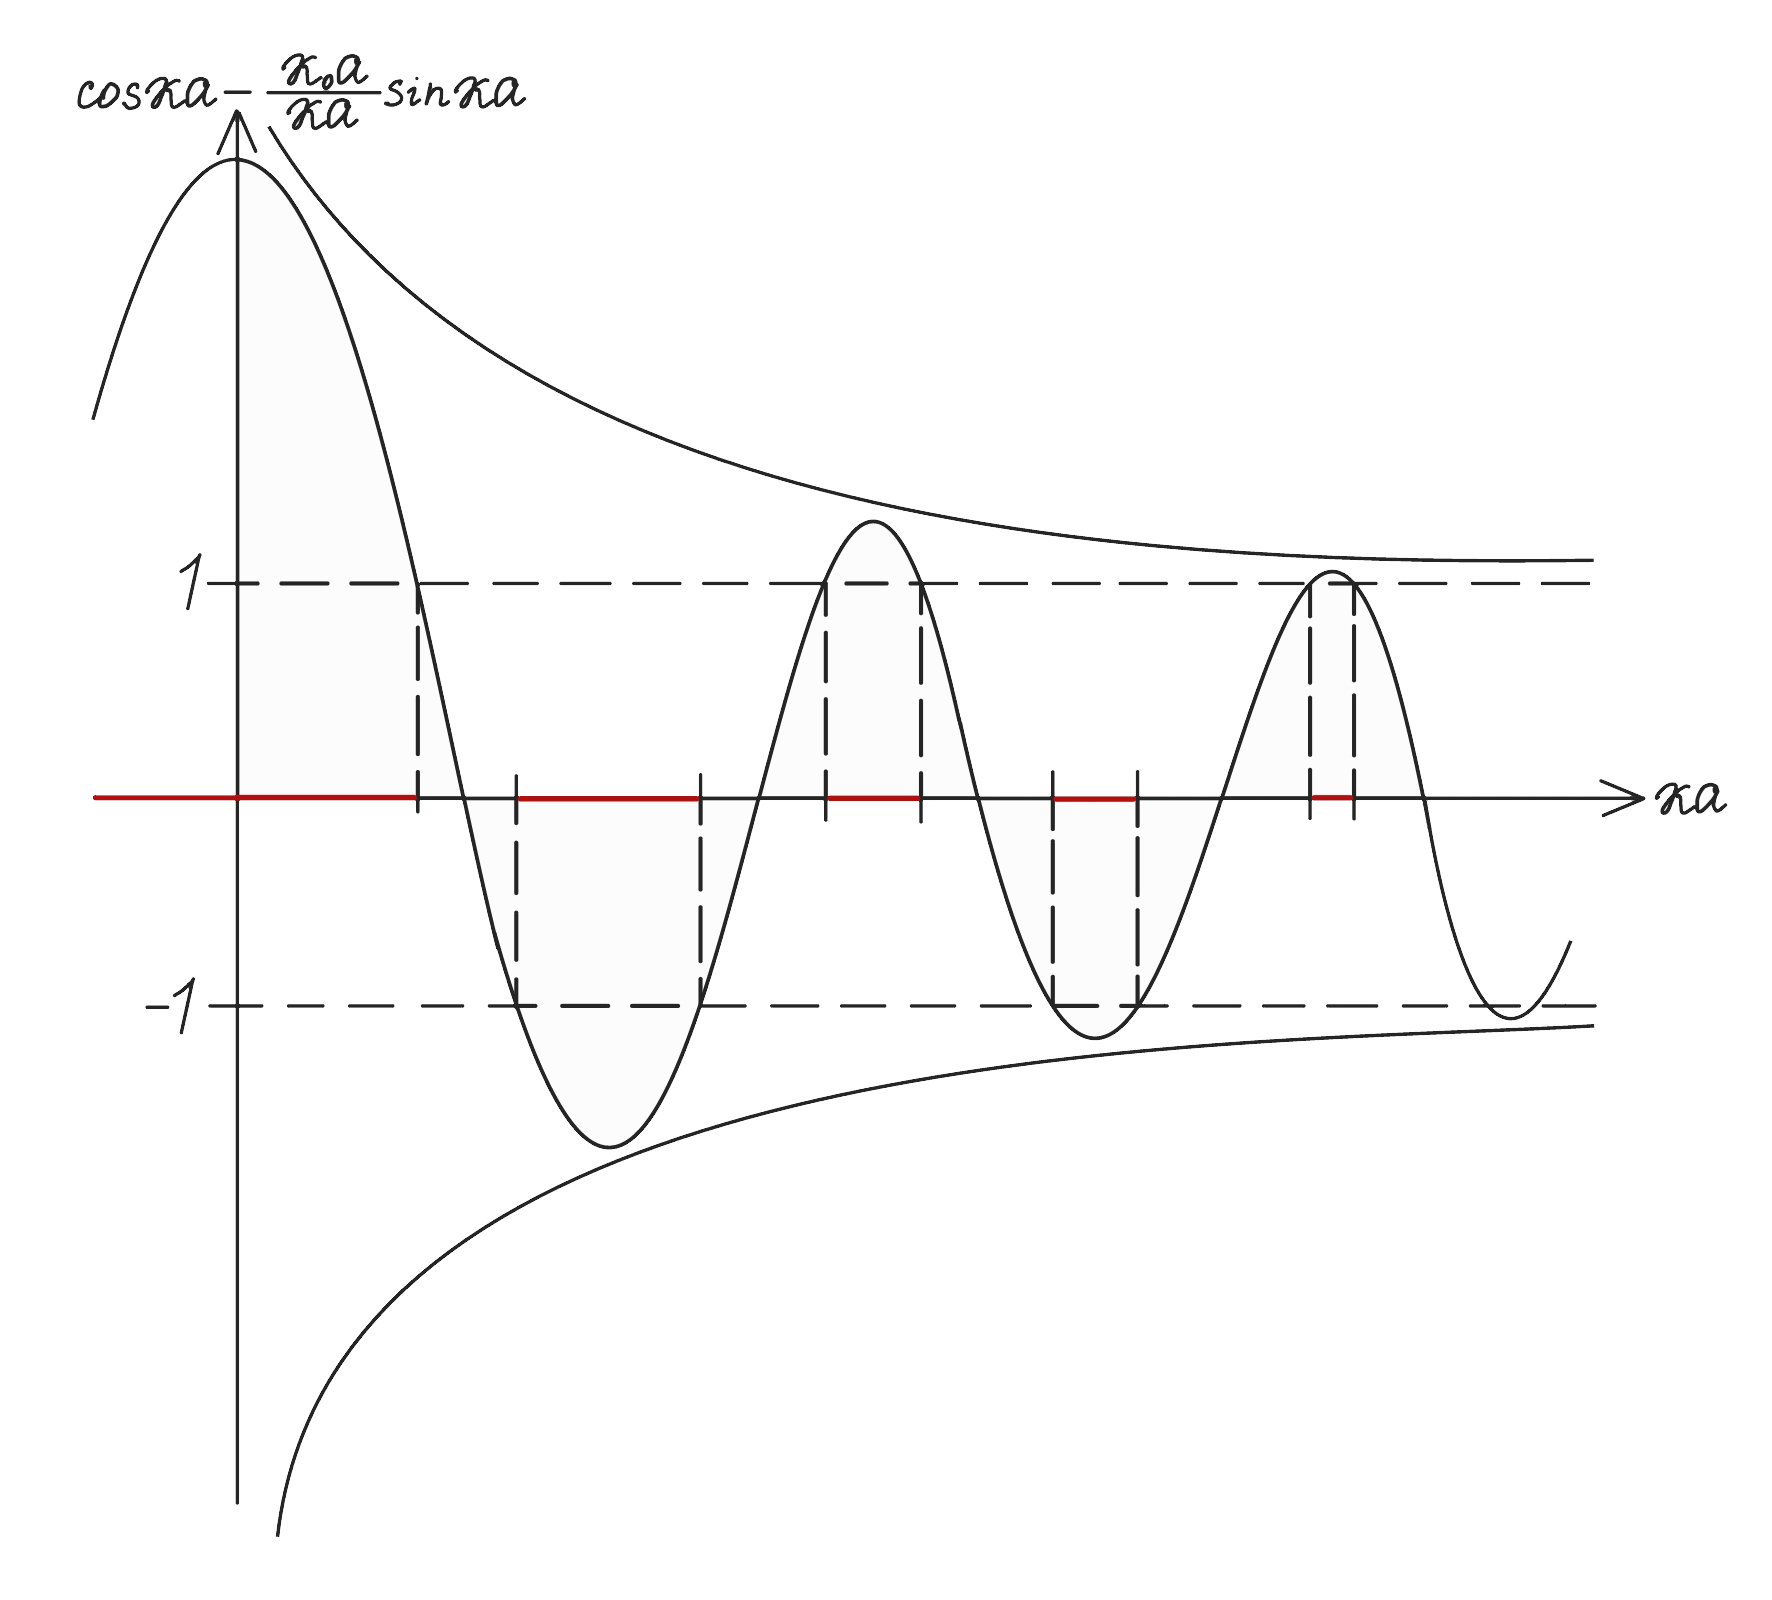
\includegraphics[scale=0.23]{class_4/images/pos energy delta.png}
\caption{График для положительных энергий}
\label{fig 4.6}
\end{figure}
Проанализируем это уравнения на графике \ref{fig 4.6}. Множитель перед косинусом указывает на вид огибающих, внутри которых будет распростроянться косинус $\cos (\kappa a + \phi)$. Так как значение k у нас действительные, косинус энергии не может выходить за пределы 1 и -1. Получается, что все зоны, когда график выходит за пределы, являются запрещёнными для энергии. И наоборот, значения внутри наших пределов будут разрешенными. Мы получили зонную структуру. Это значит, что у нас существуют область, в которых мы не сможем найти нашу систему. Анализ отрциательных энергии можно провести самостоятельно.
\csquare{darklavender}

На следующем семинаре мы с вами решим последнюю задачу на ямы и обсудим ситуацию с барьерами.